
\def\biblioref{

  "Criptografia e Segurança de Redes: Princípios e Práticas".  William
  Stallings. Editora Pearson, 4$^a$ edição, 2008.

}


\lecture{Introdução à Criptografia}{crypto}

\lecturetitle{\insertlecture}{\course}

\frame{\maketitle}


\begin{frame}{\insertlecture}
 A palavra \alert{criptografia} é proveniente do grego, {\it kryptó}
   (secreto) e {\it graphein} (escrita), e designa o estudo de métodos
   de comunicação segura (confidencial) na transmissão de mensagem,
   garantindo sua integridade.
\end{frame}

\begin{frame}{Processos}

\begin{enumerate}

\item {\bf Encriptação}: codificação do conteúdo da mensagem usando um
algoritmo de forma que somente quem tenha um código usado durante a
codificação chamado chave pode decodificá-la.

\item {\bf Decriptação}: Decodificação da mensagem encriptada (cifrada)
usando um código chamado chave, obtendo o conteúdo original da
mensagem.

\end{enumerate}

\end{frame}


\begin{frame}{Técnicas de encriptação/decriptação}

\begin{enumerate}
\item {\bf Substuição}: técnica em que as letras do texto puro são substituídas por outras 
letras, números ou símbolos.

\item {\bf Transposição}: as letras são trocadas de posição. 
\end{enumerate}

\end{frame}

\begin{frame}{Processamento do texto puro}
  O processamento do texto puro pode ser efetuado por:
  
  \begin{description}
  \item[bloco] o texto é processado em pedaços;
  \item[fluxo] o texto é processado de forma contínua.
  \end{description}

\end{frame}

\begin{frame}{Cifra de César}{Exemplo de técnica de substituição}

 Esquema antigo de criptografia atribuído ao imperador Júlio César que
consiste trocar cada letra do alfabeto por aquela que fica três
posições adiante.\bigskip

Exemplo: Oi Alice $\Rightarrow$ RL DOLFH\bigskip

\begingroup
\begin{center}
\scriptsize
\begin{tabular}{cccccccccccccc}
a& b& c &d &e &f& g &h& i& j &k & l & m\\
D& E &F& G& H &I &J& K &L &M& N & O & P\\
\end{tabular}\\\bigskip
\begin{tabular}{ccccccccccccc}
 n &o& p &q& r &s& t &u& v &w& x& y &z\\
 Q& R &S& T &U& V &W &X& Y &Z& A &B& C\\
\end{tabular}
\end{center}
\endgroup

\end{frame}

\begin{frame}{Cifra de César, cont.}{Exemplo de técnica de substituição}

Algoritmo de substituição do texto puro $p$ pela cifra $C$:\\

$$C = E(3, p) = (p+3) mod\ 26$$

Algoritmo de substituição da cifra $C$ pelo texto puro $p$:\\

$$p = D(3, C) = (p-3) mod\ 26$$

\begingroup
\begin{center}
\scriptsize
\begin{tabular}{ccccccccccccc}
0& 1& 2 &3 &4 &5& 6 & 7& 8& 9& 10 & 11 & 12\\
a& b& c &d &e &f& g & h& i& j & k &  l &  m\\
\end{tabular}\\\bigskip
\begin{tabular}{ccccccccccccc}
13& 14& 15 & 16 & 17 & 18 & 19 & 20 & 21 & 22 & 23 & 24 & 25 \\
 n&  o&  p &  q &  r &  s &  t &  u &  v &  w &  x &  y &  z \\
\end{tabular}
\end{center}
\endgroup

\end{frame}

\begin{frame}{Conceitos utilizados nos algoritmos}
  Os algoritmos de criptografia podem usar um ou vários dos conceitos
  a seguir, não estando restritos a estes:

  \begin{itemize}[<+-| alert@+>]
  \item Aritmética modular;
  \item Aritmética polinomial;
  \item Funções de {\it hash} (espalhamento);
  \item Geração de números aleatórios.
  \end{itemize}
\end{frame}

\frame{\begin{center}\LARGE Cifra Polialfabética
  \end{center}}

\lecture{Criptografia simétrica}{simmetric}

\begin{frame}{Criptografia simétrica}

\begin{center}
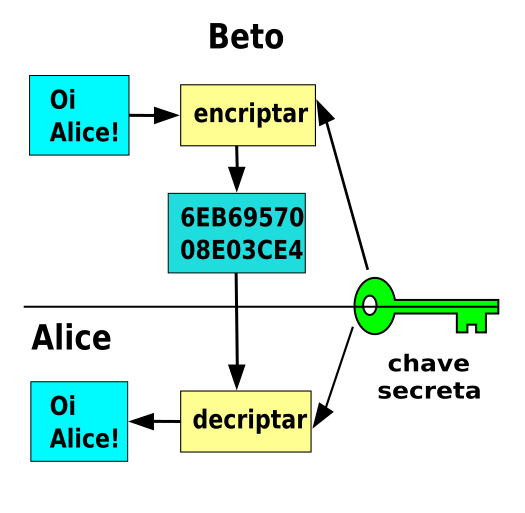
\includegraphics[scale=.4]{symmetric-key-encrypt.png}
\end{center}

\scriptsize Troca de mensagens entre Beto e Alice usando criptogtafia
simétrica. Figura adaptada de \url{https://goo.gl/Xm1GIO}

\end{frame}

\begin{frame}{Modelo de criptossistema simétrico}

Na origem, a mensagem $X$ e a chave $K$ são usados como entrada 
para o algoritmo de encriptação que produz a saída $Y$. Podemos 
escrever como

$$Y = E(K, X).$$

No destino, com a posse da chave secreta é possível realizar o caminho 
inverso, obtendo a mensagem $X$ original:

$$X = D(K ,Y).$$

\end{frame}


\begin{frame}{Uso seguro da encriptação simétrica}

\begin{itemize}
\item O algoritmo de encriptação deve ser forte, de forma que não haja
possibilidade de decriptar um texto cifrado, mesmo de posse de alguns
textos cifrados e puros usados para análise. 

\item O emissor e receptor das mensagens precisam ter obtidos cópias da
chave de uma forma segura e mantê-las protegida.
\end{itemize}

\end{frame}

\begin{frame}{Modelo de cifra simétrica}

\begin{center}
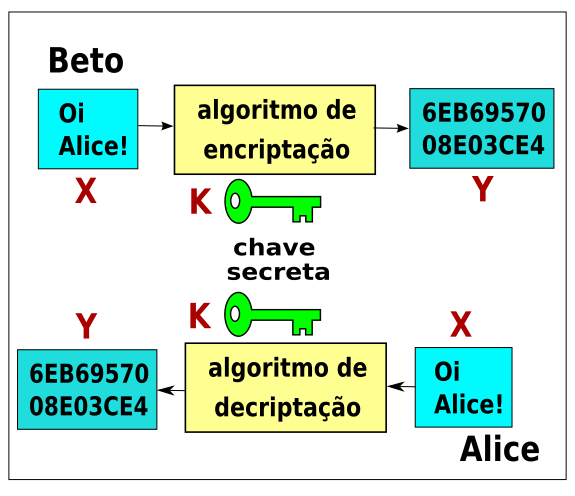
\includegraphics[scale=.4]{symmetric-cryto-model.png}
\end{center}

\scriptsize
Modelo de cifra simétrica.

\end{frame}

 \lecture{Criptografia assimétrica}{assymetric}

 \begin{frame}{Criptografia assimétrica}

 \begin{center}
 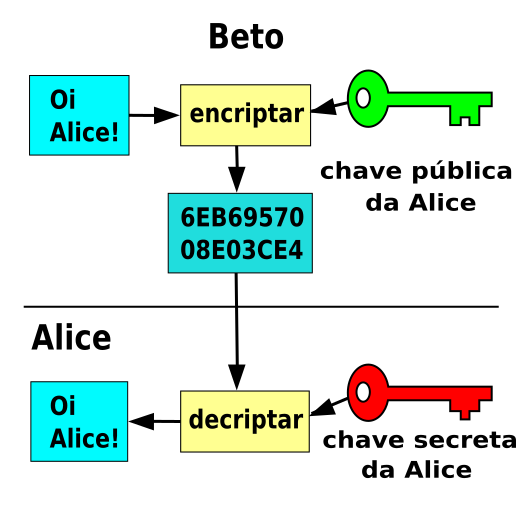
\includegraphics[scale=.4]{public-key-encrypt.png}
 \end{center}

 \scriptsize
 Troca de mensagens entre Beto e Alice usando criptogtafia de chave pública ou assimétrica. Figura adaptada de \url{https://goo.gl/jxrA5t}

 \end{frame}

\begin{frame}{Ataques}

\begin{description}

\item[For\c{c}a bruta:] testa o espa\c{c}o de possibilidades de chave e senha para tentar 
decifrar a mensagem decriptada.

\item[Criptoan\'{a}lise:] usa as falhas e brechas do sistema criptogr\'{a}fico para decriptar 
a mensagem, mesmo sem a posse da chave.
\end{description}
\end{frame}

\begin{frame}{Alguns algoritmos}{Criptografia moderna}

  \begin{itemize}[<+-| alert@+>]
  \item Cifra simétrica (chave privada)
    \begin{enumerate}
    \item DES ({\it Data Encryption Standard})
    \item AES ({\it Advanced Encryption Standard})
    \item RC4
    \item Blowfish
    \end{enumerate}

  \item Cifra assimétrica (chave pública)
    \begin{enumerate}
    \item RSA (Rivest-Shamir-Adleman)
    \item Diffie-Hellman
    \end{enumerate}

  \end{itemize}
  
\end{frame}

\ifnum1=2

\lecture{Assinatura Digital}{signature}

\frame{\title{\insertlecture}\maketitle}

\begin{frame}{\insertlecture}{Passos}
  \scriptsize

\begin{center}
  \begin{tikzpicture}[msg/.style={font=\rm,fill=yellow,text width=4cm,draw, minimum height=3cm},
    process/.style={single arrow,shape border uses incircle,text width=1.25cm,draw},
    digest/.style={font=\tiny,draw},
    label/.style={font=\scriptsize\color{gray},},
    sign/.style={fill=black,font=\color{white}}]

    \node<1>[msg] (MSG) {Oi Beto, gostaria de detalhar alguns assuntos discutidos na reunião de ontem!\\\bigskip\bigskip Alice};
    \node<1>[label] [above of=MSG,yshift=1cm] {mensagem};
    \node<1>[process,text width=1cm] (HASH) [right of=MSG,xshift=2cm] {\em hash};
    \node<1>[digest] (DIGEST) [right of=HASH,xshift=3cm] {f45d4ba0fdec254b06f41978a00a2970};
    \node<1>[label] [above of=DIGEST] {síntese da mensagem ({\em message digest})};

    \node<2>[digest] (DIGEST) [] {f45d4ba0fdec254b06f41978a00a2970};
    \node<2>[process] (ENCRYPT) [right of=DIGEST,xshift=2.75cm] {encripta com a chave privada de Alice};
    \node<2>[sign] (DIGEST) [right of=ENCRYPT,xshift=2.75cm] {Assinatura};

    \node<3,4>[msg] (MSG) {Oi Beto, gostaria de detalhar alguns assuntos discutidos na reunião de ontem!\\\bigskip\bigskip Alice};
    \node<3,4>[sign] (DIGEST) [below of=MSG] {Assinatura};
    \node<3> [label] [above of=MSG,yshift=2cm] {Concatena a assinatura na mensagem};
    \node<4>[process,font=\tiny] (DECRYPT) [right of=DIGEST,xshift=2.75cm] {Beto decripta com a chave pública de Alice};
    \node<4>[digest] (DIGEST) [right of=DECRYPT,xshift=3cm] {f45d4ba0fdec254b06f41978a00a2970};
    \node<4>[font=\tiny] [below of=DECRYPT,yshift=-1cm] {O software de Beto compara o hash da mensagem com o gerado a partir da assinatura.};

  \end{tikzpicture}

\end{center}
\end{frame}

\begin{frame}{Referência}

\biblioref

\end{frame}

\begin{frame}[fragile]{Exemplo de aplicação em Java: Chave DES}

\noindent \href{http://book.holanda.xyz/sec/src/crypto/ChavePrivadaExemplo.java}{ChavePrivadaExemplo.java}

\only<1> {
\framesubtitle{Cabeçalho}
\lstinputlisting[firstline=2,lastline=8]{src/crypto/ChavePrivadaExemplo.java}
}  


\only<2,3> {
\framesubtitle{Entrada de dados e geração da chave}
\lstinputlisting[firstnumber=10,firstline=10,lastline=16]{src/crypto/ChavePrivadaExemplo.java}
}  


\only<3> {
\framesubtitle{Cifragem e encriptação}
\lstinputlisting[firstnumber=17,firstline=17,lastline=23]{src/crypto/ChavePrivadaExemplo.java}
}  

\only<4> {
\framesubtitle{Entrada de dados e geração da chave}
  \lstinputlisting[firstnumber=24,firstline=24,lastline=35]{src/crypto/ChavePrivadaExemplo.java}
}  

\only<5> {
  \framesubtitle{Decriptação}
   \lstinputlisting[firstnumber=36,firstline=36,lastline=44]{src/crypto/ChavePrivadaExemplo.java}
}  



\end{frame}

\begin{frame}[fragile]{Exemplo de aplicação em Java: Chave pública RSA}

\noindent \href{http://book.holanda.xyz/sec/src/crypto/ChavePublicaExemplo.java}{ChavePublicaExemplo.java}

\only<1> {
\framesubtitle{Cabeçalho}
\lstinputlisting[firstline=2,lastline=9]{src/crypto/ChavePublicaExemplo.java}
}  


\only<2,3> {
\framesubtitle{Entrada de dados e geração da chave}
\lstinputlisting[firstnumber=10,firstline=10,lastline=16]{src/crypto/ChavePublicaExemplo.java}
}  


\only<3> {
\framesubtitle{Cifragem e encriptação}
\lstinputlisting[firstnumber=17,firstline=17,lastline=23]{src/crypto/ChavePublicaExemplo.java}
}  

\only<4> {
\framesubtitle{Entrada de dados e geração da chave}
  \lstinputlisting[firstnumber=24,firstline=24,lastline=35]{src/crypto/ChavePublicaExemplo.java}
}  

\only<5> {
  \framesubtitle{Decriptação}
   \lstinputlisting[firstnumber=36,firstline=35,lastline=44]{src/crypto/ChavePublicaExemplo.java}
}  

\end{frame}


%%%%%%%%%%%%%%%%%%%%%%%% CRYPTO ALGORITHMS %%%%%%%%%%%%%%%%

\lecture{Algoritmos de Criptografia}{cryptoalg}

\lecturetitle{\insertlecture}{\course}
\frame{\maketitle}

\begin{frame}{RSA}{Introdução}

Ron \alert{R}ivest, Adi \alert{S}hamir, Leonard \alert{A}dleman, 1977.

\begin{center}
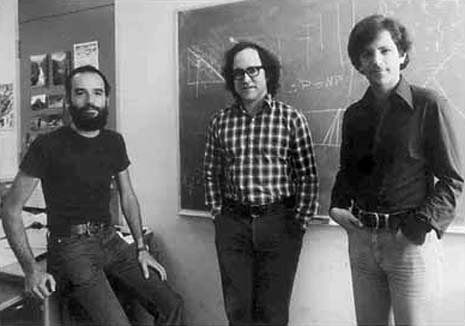
\includegraphics[scale=.4]{img/rsa.png}
\end{center}

\end{frame}

\begin{frame}{RSA}{Algoritmo}\footnotesize

  \hfil {\color{blue}\bf Geração de chave por Alice}
  
\begin{tabbing}
  Selecione $p$ e $q$ \hspace{3.3cm}\= $p$ e $q$ são primos e $p\neq q$\\
  Calcule $n=p\times q$\\
  Calcule a função totiente em $n$\> $\phi(n) = (p-1)(q-1)$\\
   Selecione o inteiro $e$ \> $mdc(\phi(n),e)=1; 1<e<\phi(n)$\\
   Calcule $d$ \> $d\equiv e^{-1}(\text{mod}\ \phi(n))$\\
   Chave pública \> $k_{\text{pública}}=\{e,n\}$\\
   Chave privada \> $k_{\text{privada}}=\{d,n\}$\\
\end{tabbing}

\pause

\hfil {\color{blue}\bf Encriptação por Beto usando a chave pública da Alice}
\begin{tabbing}
  Texto puro $M$ \hspace{3.3cm}\= $M<n$\\
  Texto cifrado \> $C = M^e \text{mod}\ n$\\
\end{tabbing}

\pause

\hfil {\color{blue}\bf Decriptação pela Alice usando sua chave privada}
\begin{tabbing}
  Texto cifrado $C$ \hspace{3.3cm}\= $M<n$\\
  Texto puro \> $M = C^d \text{mod}\ n$\\
\end{tabbing}

\end{frame}

\begin{frame}{RSA}{Exemplo}\footnotesize

  \hfil {\color{blue}\bf Geração de chave por Alice}
\begin{tabbing}
  Selecione $p$ e $q$ \hspace{3.3cm}\= $p=17$ e $q=11$\\
  Calcule $n=p\times q$ \> $n=17\times 11=187$\\
  Calcule a função totiente em $n$\> $\phi(n) = (17-1)(11-1)=16\times 10=160$\\
  Selecione o inteiro $e$ primo de $160$ \> $e=7\Rightarrow\quad mdc(160,7)=1,\quad 1<e<\phi(n)$\\
  Calcule $d$, {$\quad$\tiny assumindo $k=1$}  \> $ d.e = k.\phi(n) + 1  \Rightarrow d = \frac{1.160 + 1}{7} \Rightarrow d = 23 $\\
  Chave pública \> $k_{\text{pública}}=\{7,187\}$\\
  Chave privada \> $k_{\text{privada}}=\{23,187\}$\\
\end{tabbing}

\pause

 {\color{blue}\bf Encriptação do texto $M=88$ por Beto usando a chave pública da Alice}
\begin{tabbing}
  Texto puro $88$ \hspace{3.3cm}\= $88<187$\\
  Texto cifrado \> $C = M^e \text{mod}\ n = 88^7 \text{mod}\ 187 = 11$\\
\end{tabbing}

\pause

\hfil {\color{blue}\bf Decriptação pela Alice da cifra $C=11$ usando sua chave privada}
\begin{tabbing}
  Texto cifrado $C$ \hspace{3.3cm}\= $C<n$\\
  Texto puro \> $M = C^d \text{mod}\ n = 11^{23} \text{mod}\ 187 = 88$\\
\end{tabbing}
  
\end{frame}

\begin{frame}{RSA}{Segurança}\footnotesize
  Técnicas de ataque do algoritmo RSA:
  \begin{description}[<+->]\setbeamercovered{transparent}
  \item[Força bruta:] tentar todas as chaves possíveis.
  \item[Matemático:] a maioria das técnicas matemáticas envolve 
    fatorar o produto de dois primos.
  \item[Temporização:] analisam o tempo de execução do algoritmo de 
    decriptação.
  \item[Baseados em falha de hardware:] indução de falha de hardware durante 
    o processo de geração das chaves.
  \end{description}
  
\end{frame}

\begin{frame}{RSA}{Discussão}\footnotesize

  \begin{itemize}[<+->]\setbeamercovered{transparent}
  \item O algoritmo de \alert{Diffie-Hellman} também pode ser usado como 
    algoritmo de chave assimétrica.
  \item É recomendado que o número de bits para o RSA seja pelo menos 2.048.
  \item Como os primos $p$ e $q$ devem ser números muito grandes para
    dificultar a fatoração, uma biblioteca matemática para manipulação
    de inteiros com precisão arbitrária deve ser usada, por exemplo, a
    \href{https://wiki.openssl.org/index.php/Manual:Bn_internal(3)}{\tt
      BIGNUM} que vem com o OpenSSL ou a
    \href{https://gmplib.org/}{GNU de precisão múltipla ({\tt gmp})}.

\item Também é importante utilizar um biblioteca que gere ``bons'' 
  números aleatórios.
  \end{itemize}

\end{frame}

\begin{frame}{Referência}

\begin{itemize}
\item \biblioref

\item ``Secure Programming Cookbook''. John Viega e Matt
  Messier. O'Reilly, 2003.

\end{itemize}

\end{frame}
\fi